\cotefile{85}
\scanpage{30}
conclut le résultat \unsure{analogue} sans restr. sur les
car. résiduelles, car le schéma des \deleted{\unsure{élém.|éléments}} ``réflexions''
dans $\mathrm{GP}(1)_{\mathbb Z}$ est lisse sur $\mathrm{Spec}\,\mathbb Z$. Dans le cas d'
une forme de $\mathrm{Sl}(2)$, OPS que c'est $\deleted{\unsure{\mathrm{Sl}_2|\mathrm{Sl}}}\,(V)$, \deleted{\unsure{donc|i.e.}} \inserted{i.e.}
$u$ est un autom. de $V$ satisfaisant $\deleted{\unsure{u^2=\mathrm{id}}},\ \det u=1$,
\deleted{Mais $u_s\ne\mathrm{id}\quad\forall s\in S$} \unsure{Car|Comme} \deleted{\unsure{donc}} par Hamilton-Cayley
\deleted{\unsure{Tr}}, $u^2-(\mathrm{Tr}\,u)u+1\mathrm{id}=0$, donc $\inserted{u^2=\mathrm{id}\Longleftrightarrow}(\mathrm{Tr}\,u)u=2\mathrm{id}$, \deleted{pour que} \inserted{de cette hyp.}
\deleted{$u^2=\mathrm{id}$, comme $u$ est} il faut conclure ``$\mathrm{Tr}\,u=-2$''. Faisant un calcul infinitésimal,
\deleted{on trouve par erreur que ça coince, d'où \unsure{le}} \deleted{pour en conclure que} \deleted{\unsure{sauf}} aucune solution en
\deleted{nécessité de cette restriction. --}
car. résiduelle 2, OPS qu'on a $\mathrm{Tr}\,u_n=-2$, et \inserted{on va essayer} prouver
$\mathrm{Tr}\,u_{n+1}=\mathrm{Tr}\,u=-2$. \deleted{On aura $\mathrm{Tr}\,u+2=\tau$ avec $\unsure{m\tau}=0$}

% slanted
\margin{\unsure{bien peu|bien au} clair\unsure{…}}

\uline{Proposition} Soit $G$ une forme de $\mathrm{GP}(1)_S$ ou $\mathrm{Sl}(2)_S$, $u$ une
section de $G$, \inserted{$\alpha=A(u)$,} \deleted{telle que $(A(u)+2)(A(u)-2)$ soit inv.,}
$n$ un entier $\geq3$. \deleted{Pour que l'on ait \unsure{Soit $F_n$|Soient $F_n$}} \inserted{On suppose $(\alpha+2)(\alpha-2)$ inv.} Soient

\[
\begin{aligned}
F_n&\in\mathbb Z[U]\\ 
\Psi_n&\in\mathbb Z[U]
\end{aligned}
\]

les deux polynômes \deleted{que} unitaires \deleted{\unsure{sur}} \inserted{à racines deux à deux distinctes} dont les
racines sont 1°) $\zeta+\zeta^{-1}$, où $\zeta$ parcourt les racines
$n$-ièmes \deleted{de} de $1$ \deleted{telles} distinctes de $\pm1$ \enspace 2°) les $\zeta+\zeta^{-1}$,
où $\zeta$ parcourt les racines \uline{primitives} $n$-ièmes de $1$\unsure{.}

\deleted{Pour q}\inserted{Sous ces conditions}

Pour que, $u^n=\mathrm{id}$, il f. et s. que $F_n(\alpha)=1$

Pour que \inserted{on ait} $u^n=\mathrm{id}$ et que $u_s$ soit d'ordre $n$
exactement pour tt $s\in S$, il f. et s. que $\Psi_n(\alpha)=0$.

% slanted
\margin{Sans l'hyp. préalable que $\alpha^2-4$ inv., on peut dire que $[u^n=\mathrm{id}$ et les $u_s$ d'ordre $n$ exactement et $n$ premier aux car. résiduelles$]$ $\Longleftrightarrow$ $[\deleted{\unsure{F}}\Psi_n(\alpha)=0$ \uline{et} $\alpha^2-4$ inv.$]$,}

Principe de démonstration. L'hyp. $\deleted{\alpha^2\ne}\inserted{\alpha\unsure{-|\ne}2}$ inv.
\inserted{i.e. les $u_s$ non unipotents,} implique déjà l'existence d'un unique tore maximal
$T$ qui contient $u$. OPS $T\simeq\mathbb G_m$, donc $u$ donné par une

% archive sheet number: 29
\scanpage{31}
section $\lambda$ de $\mathbb G_m$, donc \deleted{\unsure{$\alpha$|$*$}}

\[
\alpha=\lambda+\lambda^{-1},
\]

et on est ramené à une question de calcul
standart.

\deleted{Pour \unsure{analyser}}

\uline{Cor. 1} Supposons les car. résiduelles de $S\ne3$. Pour qu'
une section $u$ de $G$ satisfasse $u^3=\mathrm{id}$ (resp. $u^6=\mathrm{id}$) et que
l'ordre de $u_s$ ($s\in S$) soit tjrs égal à 3 (resp 6) il f et s.
qu'on ait $\alpha=-1$ (resp. $\alpha=+1$).

\deleted{\unsure{L'une et l'autre hyp. signifie que|L'une et l'autre hyp. implique que}}

\uline{Cor 2} Supposons les car. rés. de $S\ne2$. Pour que l'on
ait $u^4=\mathrm{id}$ et que les $u_s$ $(s\in S)$ soient d'ordre 4 exactement,
il f. et s. que $\alpha=0$

\uline{Cor. 3} Supposons les car. résiduelles $\ne5$. Pour que
$u^5=0$ et les $u_s$ d'ordre 5, il f et s. qu'on ait

\[
\alpha^2+\alpha-1=0
\]

\uline{NB} L'ordre \inserted{$\nu$} d'un élément $\tilde u$ de $\mathrm{Sl}(2,k)$ ($k$ un corps)
-- donc d'un $\widetilde G(k)$ pour une forme \inserted{$\widetilde G$} de $\mathrm{Sl}(2)$ \unsure{sur|sur $k$}
\deleted{\unsure{ou}} peut être d'une des formes suivantes \deleted{\unsure{ou $p$}}
pour une car. donnée

a) \inserted{$\nu=$} $+\infty$\\ 
b) $\nu$ entier $\geq1$ \uline{premier à} $p$ :\\ 
c) $\nu=2p$ ($p$ premier \uuline{impair})\\ 
\deleted{\unsure{multiple de $p$}}\\ 
d) $\nu=p$
\margin{si $p=\mathrm{car.}\,k$ est \unsure{finie|impair|fini} $\Big\}$}

Si on exclut les cas $\pm\mathrm{id}$ (élémt du centre, i.e.
d'un élément qui donne $1$ dans $\widetilde G/\mu_2=G$)
[qui donnent lieu à $\alpha=\pm2$, mais d'autres cas y
donnent lieu aussi] on a vu que la valeur
de $\alpha$ détermine (loc. fppf) la classe de conj. de
$u$. On trouve en fait l'analyse suivante :

% archive sheet number: 30
\scanpage{32}
% archive sheet number: 31

\deleted{$\nu$ \uline{premier à $p$} ($p$ fini) $\longleftrightarrow$}

% slanted
\margin{On suppose \uuline{$u$ \deleted{\unsure{$\ne$}}non central}}

% slanted
\margin{$\zeta$ une solution de $\zeta^2-\alpha\zeta+1=0$ dans $\bar k$}

$k$ \uline{car. 0} \uline{($p=+\infty$)}

\[
\begin{aligned}
\deleted{\unsure{A)|a)}}\quad \nu\ \text{fini}&\Longleftrightarrow\exists\,\deleted{\unsure{n}}\inserted{n\geq3}\ \text{tel que }\Psi_n(\alpha)={}\\ 
\deleted{\unsure{B)|b)}}\quad\text{''}&\Longleftrightarrow \deleted{\zeta\ \text{racine}}\ \zeta\ \text{d'ordre fini }\ne1,2
\end{aligned}
\]

$k$ car. $p>0$

\[
\begin{aligned}
\mathrm A)\quad\nu\ \text{fini}&\Longleftrightarrow\alpha\ \text{algébrique}\Longleftrightarrow n\geq1\ \text{tel}\\ 
&\hspace{4em}\text{que }\Psi_n(\alpha)=0\ (\\ 
&\Longleftrightarrow\exists\,n\geq1,\ \text{premier à }p\\ 
&\hspace{3em}\text{ou de la forme }\deleted{\unsure{2}}2p,\\ 
&\hspace{3em}\deleted{\unsure{\text{ou }2p\ (\text{avec}|2p\ (\text{avec}}}\ p\ \text{impair})\\ 
&\hspace{3em}\inserted{\text{ou }p,}\ \text{tel que }\Psi_n(\alpha)=0\\ 
(S\ne\varnothing)&\quad[\text{ledit }n\ \text{étant alors}\\ 
&\hspace{3em}\text{unique, et égal à }\nu(u)]\\ 
&\Longleftrightarrow\zeta\ \text{d'ordre fini. En fait,}\\ 
&\hspace{2em}\text{si}
\end{aligned}
\]

\uline{Théorème} $\widetilde G$ forme de $\mathrm{Sl}(2)_S$, $u$ section de $\widetilde G$, $\alpha=A(u)\in\Gamma(S,\unsure{\mathcal O_S|\frac{\mathcal O}{S}|\underline{O}_S})$,
$n\in\mathbb N$, $\boxed{n\geq3}$. On s'intéresse à la traduction, en termes de $\alpha$,
et de propriétés des car. résiduelles de $S$, de la propriété
suivante

% slanted
\margin{\uline{NB} On ne permet pas $n=2$, qui \unsure{compliquerait|cancellerait|se calculerait} complètement}

\[
(*)\quad u^n=\mathrm{id},\quad\text{et }\forall s\in S,\ \text{l'ordre de }u_s\ \text{est égal à }n.
\]

A) Supposons que $n$ ne soit \deleted{ni un nb premier, ni} \inserted{de la forme $p$ \inserted{ni $2p$} ($p$ premier}
\deleted{ni $2p$ ($p$ premier)} \deleted{impair} \uline{impair}). Alors $(*)$ équivaut à :

a) $\Psi_n(\alpha)=0$, et $n$ inv. sur $S$ (i.e. les car résiduelles
sont premières à $n$)

% slanted
\margin{\uline{NB} le cas $n=4$ \unsure{est pas|n'est pas} exclu -- A) doit marcher pareil ds le cas de $G=\widetilde G/\mu_2$}

B) $n=2p$ ($p$ premier impair). Alors $(*)$ équivaut à :

b) $\Psi_n(\alpha)=0$, et $2$ inv sur $S$ (i.e. car. rés. de $S$
sont $\ne2$)

% slanted
\margin{\uline{à vérifier} $\left.\vphantom{\Large A}\right\}$ Peut-être faux (\unsure{bon entraînement|bien certainement|bons contre-exemples} \unsure{faites sur papier|faux si non premier}…)}

C) $n=p$, $p$ est premier \inserted{impair}. Alors $(*)$ équivaut à :

c) $\Psi_n(\alpha)=0$.

\uline{NB} Ces conditions \uline{n'impliquent pas} $(\alpha+2)(\alpha-2)$ inv, sauf ds le cas A
Dans les cas B \deleted{resp. C} \inserted{et C}, les pts où $\alpha_s^2-4=0$ sont ceux de car $p$,
\deleted{(où $\alpha_s=-2\ne2$] (resp. ceux de car} où $\alpha_s=-2\ne+2$ (cas B) resp $\alpha_s=+2\ne-2$ (cas C)
\scanpage{33}
(8 p)

Sous-groupes finis de
$\mathrm{GP}(1)$

% archive sheet number: 32
\scanpage{34}
\uline{Sous-groupes finis de} $\mathrm{GP}(1,k),\mathrm{Sl}(2,k),\mathrm{Gl}(2,k)$

On suppose d'abord $k$ corps de car. 0, alg clos.

a) \uline{Sous groupes finis de} $\mathrm{GP}(1,k)=G$

\uline{Thme} a) Pour que deux ss-groupes finis \inserted{$\Gamma,\Gamma'$} de $G$ soient conjugués
dans $G$, il f. et s. qu'ils soient isomorphes.

b) Les classes d'isom. de sous-groupes finis de $G$
sont \inserted{celles de} $\mathbb Z/n\mathbb Z$ ($n\deleted{\unsure{\geq1}}\deleted{\unsure{\geq2}}$), $\mathbb D_n$ ($n\geq2$), $\mathcal A_4,\unsure{\mathfrak S_4|\mathscr S_4},\mathcal A_5$, i.e.
ce sont \uline{exactmt} les types des groupes d'isom. des
\inserted{cartes orientées régulières sphériques (avec leurs \uline{plongements} naturels ds $\mathrm{GP}(1)$\unsure{.…})}

% slanted

\deleted{c) Si $\Gamma$ est un sous-gpe de $G$, son normalisateur}
\deleted{il est égal à son normalisateur, sauf dans les
cas de $\mathbb Z/n\mathbb Z$ ($n\geq1$) et de $\mathbb D_2$, \inserted{de $\mathcal A_4$.} Dans ces cas
on a, notant à part le cas trivial de $1=\mathbb Z/n\mathbb Z$ \unsure{on a :|inclus :}}
\deleted{on a}

\deleted{1°) \deleted{Normalisateur de} $N(\mathbb Z/n\mathbb Z)$ \deleted{est} \deleted{le normali}\inserted{$N(T)$}, $T=Z(\mathbb Z/n\mathbb Z)$
est l'unique tore maximal qui cont.
$\mathbb Z/n\mathbb Z$, \deleted{Centr.} $N(\mathbb Z/n\mathbb Z)/Z(\mathbb Z/n\mathbb Z)=\mathbb Z/2\mathbb Z$}

\deleted{2°) \deleted{Normalisateur de} $N(\mathbb D_2)\unsure{\Rightarrow|=|\xrightarrow{\sim}}\mathfrak S_4$,}

\[
\begin{aligned}
&\deleted{\text{Centralisateur de}}\quad\deleted{Z(\mathbb D_{\unsure{2|n}})=\mathbb D_2}\\ 
&\deleted{N(\mathbb D_2)/Z(\mathbb D_2)\xrightarrow{\sim}\mathrm{Aut}(\mathbb D_2)\simeq\mathfrak S_3}
\end{aligned}
\]

\[
\begin{aligned}
&\deleted{3^\circ)\quad N(\mathcal A_4)=\mathfrak S_4}\\ 
&\deleted{Z(\mathcal A_4)=(1)}\qquad\deleted{N(\mathcal A_4)/Z(\mathcal A_4)=\mathfrak S_4}\\ 
&\hspace{14em}\deleted{=\mathrm{Aut}(\mathcal A_4)}
\end{aligned}
\]

\figure{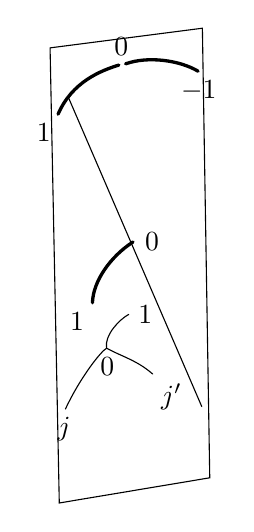
\begin{tikzpicture}[x=.78cm,y=.78cm,line cap=round]
\draw (-.48,6.38)--(2,6.7)--(2.12,-.62)--(-.33,-1.03)--cycle;
\draw[very thick] (-.35,5.3) .. controls (-.12,5.83) and (.35,6.01) .. (.64,6.1);
\draw[very thick] (.75,6.12) .. controls (1.11,6.25) and (1.63,6.18) .. (1.93,6.0);
\node[below left] at (-.31,5.30) {$1$}; \node[above] at (.68,6.09) {$0$}; \node[below] at (1.94,6.0) {$-1$};
\draw[very thick] (.21,2.23) .. controls (.22,2.58) and (.50,2.98) .. (.87,3.22);
\node[below left] at (.23,2.23) {$1$}; \node[right] at (.91,3.22) {$0$};
\draw (-.23,.5) .. controls (.02,1.03) and (.35,1.44) .. (.44,1.49) .. controls (.70,1.35) and (.94,1.29) .. (1.19,1.07);
\draw (.44,1.49) .. controls (.4,1.70) and (.65,1.96) .. (.80,2.04);
\node[below] at (.45,1.50) {$0$}; \node[right] at (.8,2.04) {$1$}; \node[below] at (-.25,.53) {$j$}; \node[below right] at (1.17,1.07) {$j'$};
\draw[thin] (-.18,5.57)--(1.99,.54);
\end{tikzpicture}}

\deleted{D'autre part, dans tous les cas sauf}

\deleted{c) Pour toute carte \deleted{\unsure{$G$}} orientée finie
sphérique (connexe) $\mathcal C$, considérons sa
réalisation topologique -- on trouve un
foncteur de groupoïdes}

\diagram{\begin{tikzcd}[ampersand replacement=\&,column sep=small]
\deleted{\mathcal C}\arrow[r,"{\deleted{\unsure{\sim}}}"]\&\deleted{\substack{\mathcal C=\text{cat. des}\\ \text{``cartes holomorphes sphériques'',}\\ \text{i.e. des ``cartes h.\unsure{lomorphes}''}\\ \deleted{\text{sur}}\ \text{telles que la variété}\\ \text{complexe sous-jacente}\\ \text{soit }\deleted{\text{de}}\ \unsure{\text{simple}|\text{sphère}|\text{de type}}\ \text{de genre 0}}}\arrow[r]\&\deleted{\substack{\text{catégorie}\\ \text{des couples}\\(G,\Gamma)\ \text{d'une}\\\text{forme de}\\\mathrm{GP}(1,\mathbb C)\\\text{et d'un}\\\text{sous-gp.}\\\text{fini }\Gamma}}
\end{tikzcd}}

% archive sheet number: 33
\scanpage{35}
1) Soit $\Gamma\simeq\mathbb Z/n\mathbb Z$, $n\geq2$. Alors
$T=Z(\Gamma)$ est un tore maximal de $G$, et c'est l'unique
tore maximal de $G$ contenant $\Gamma$. On a \deleted{\unsure{et}} $\Gamma={}_nT$,
\deleted{$N(\Gamma)=$}
et les applications $\Gamma\mapsto T=Z(\Gamma)$, $T\mapsto{}_nT=\Gamma$,
définissent des bijections inv. l'une de l'autre
entre l'ens des tores maximaux de
$G$, et l'ens des ss-gpes de $G$ \deleted{\unsure{dér $Z$}}
cycliques d'ordre $n$. \quad ($\Rightarrow$)

\figure{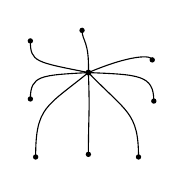
\begin{tikzpicture}[scale=.67,line cap=round]
\foreach \a/\b/\c/\d in {-1.1/.6/-1/.2,-1.1/-.5/-.9/-.05,-1/-1.6/-.8/-.65,0/-1.55/.03/-.8,.95/-1.6/.72/-.75,1.24/-.54/.95/-.04,1.21/.24/.8/.34,-.12/.80/.02/.60}{
\draw (0,0) .. controls (\c,\d) and (\a,\d) .. (\a,\b); \fill (\a,\b) circle(1.45pt);}
\fill (0,0) circle(1.6pt);
\end{tikzpicture}}

\[
\inserted{\mathrm{Aut}(G,\Gamma)\simeq}N(\Gamma)=\deleted{\unsure{\mathrm{Aut}(G,\Gamma)=|\mathrm{Aut}(G,T)=}}N(T)\deleted{=},\qquad N(\Gamma)/Z(\Gamma)=\mathrm{Aut}(G,\Gamma)\simeq\mathbb Z/2\mathbb Z
\]

\diagram{\begin{tikzcd}[ampersand replacement=\&,row sep=small]
\mathrm{Aut}\,\Gamma\\ 
\mathbb Z/2\mathbb Z\arrow[u,hook]
\end{tikzcd}}

\margin{\uline{NB} 1° et 3° sont les seuls cas abéliens}
\margin{\unsure{devant} $\longleftarrow$}

\uline{Corollaire} La donnée, sur un schéma $S$ de car. 0, d'une
forme $G$ de $\mathrm{GP}(1)$ et d'un sous-gpe étale fini $\Gamma$ de $G$,
cyclique d'ordre $n$ ($n\geq2$ donné), équivaut à celle d'une \unsure{Module dté|Module|Mod.}
\unsure{quadratique} \unsure{lisse} de rg 2 sur $S$.

% slanted
\margin{\unsure{expliciter} les foncteurs}

3) Soit $\Gamma=\mathbb D_2\inserted{=\mathbb Z_2\times\mathbb Z_2}$. Alors

\[
Z(\Gamma)=\Gamma
\]

$N(\Gamma)=\unsure{\mathfrak S_4|\mathscr S_4}$, $N(\Gamma)$ est l'unique ss-gpe de type
$\mathcal A_4$ qui contienne $\Gamma$, et $\Gamma\mapsto N=N(\Gamma)$,
$N\longmapsto\Gamma={}$ unique ss-gpe de type $\mathbb D_{2}$ de
$N$ $={}$ unique ss-gpe invariant ``\deleted{propre}'' \deleted{de}
de $N$ distinct de $[N,N]$ i.e. d'indice
$\ne2$ [ou encore d'indice 6], sont des
corr. 1-1 entre l'ens des sous-gpes
de $G$ de type $\mathbb D_2$, et l'ens des ss-gpes de type $\mathfrak S_4$.

\figure{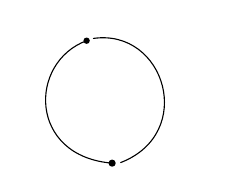
\begin{tikzpicture}[scale=.72,line cap=round]
\draw (-.35,1.08) .. controls (-1.38,.7) and (-1.38,-.96) .. (.10,-1.08);
\draw (.25,-1.07) .. controls (1.59,-.55) and (1.03,1.30) .. (-.23,1.12);
\fill (-.35,1.08) circle(1.6pt);\fill (.10,-1.08) circle(1.8pt);
\end{tikzpicture}}

\margin{\uline{NB} Ici $N(\Gamma)\to\mathrm{Aut}(\Gamma)$ non injectif (c'est le seul cas, avec le cas}

\[
N(\Gamma)/Z(\Gamma)\ \mathrel{\overset{\sim}{\rule{1.5em}{.4pt}}}\ \mathrm{Aut}(\Gamma)\simeq\mathfrak S_3
\]

\uline{Corollaire} La donnée d'un ss-groupe

\uline{Corollaire} \inserted{Sur base $S$ de car. 0,} la donnée d'un $(G,\Gamma)$, $G$ forme
de $\mathrm{GP}(1)$, \deleted{\unsure{$\Gamma\subset D_2$}} $\Gamma\subset G$ forme de $\mathbb D_2$, équivaut
à celle de $(G,\widetilde\Gamma)$, $G\ldots$, $\widetilde\Gamma\subset G$ forme de
$\mathfrak S_4$, ou encore à celle d'un torseur
sous $\mathfrak S_4$, ou encore d'un rev. étale de
degré 4 de $S$, ou celle d'un \uline{tétraèdre} sur $S$.

\margin{ou celle de \uline{octaèdre} \uline{\unsure{Orienté|Orientés}} sur $S$.}

% archive sheet number: 34
\scanpage{36}
\margin{\unsure{permuter|puis --} $\longleftrightarrow$}

2) Soit $\Gamma=\mathbb D_n$ \uline{($n\geq3$)}, \deleted{Alors} $\inserted{\Gamma^+\simeq\mathbb Z/n\mathbb Z}$ le ss-gpe car. d'indice 2,
$T=\inserted{Z(\Gamma^+)}$ l'unique tore maximal qui

\[
\begin{aligned}
Z(\Gamma)&=\deleted{\unsure{\mathbb D}}\deleted{\unsure{\{1\}}}\,{}_2T\simeq\{\pm1\}\\ 
\inserted{\mathrm{Aut}(G,\Gamma)=}N(\Gamma)&=\begin{cases}\Gamma&\text{si }n\text{ pair}\\ \Gamma\cdot{}_2T&\text{si }n\text{ impair}\end{cases}\\ 
N(\Gamma)/Z(\Gamma)&\ \deleted{\unsure{\simeq N}}\deleted{\unsure{=\mathrm{Aut}(\Gamma)|\simeq\mathrm{Aut}(\Gamma)}}\ \inserted{\unsure{\simeq}}\ \Gamma/{}_2\Gamma^+\overset{\deleted{\unsure{\sim}}}{\subset}\mathrm{Aut}(\Gamma)
\end{aligned}
\]

\margin{\uline{vérifier}}

\figure{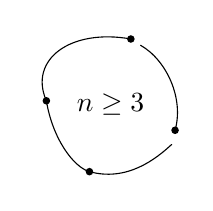
\begin{tikzpicture}[scale=.72,line cap=round]
\draw (.36,1.21) .. controls (-.7,1.4) and (-1.45,.85) .. (-1.13,.12) .. controls (-1.02,-.55) and (-.65,-1.05) .. (-.37,-1.13) .. controls (.29,-1.31) and (.80,-.91) .. (1.08,-.65);
\draw (.53,1.10) .. controls (.99,.84) and (1.30,.16) .. (1.14,-.40);
\foreach \x/\y in {.36/1.21,-1.13/.12,-.37/-1.13,1.14/-.40}{\fill (\x,\y) circle(1.9pt);}
\node at (0,.05) {$n\geq3$};
\end{tikzpicture}}

\uline{Corollaire} \inserted{Sur $S$ sch de car. 0, si $n$ pair} La cat. des $(G,\Gamma)$, $G$ forme de
$\mathrm{GP}(1)$, $\Gamma\subset G$ \deleted{ss-gpe fini ét.} \inserted{forme de $\mathbb D_n$} ($n$ fixé $\geq\unsure{4|3}$)
équivaut à celle des rev. principaux de
$S$ de gpe $\mathbb D_n$, \deleted{\unsure{ou}} ou à celle des \uline{polygones}
réguliers sur $\underline S$ de degré $n$.

% slanted
\margin{\deleted{\unsure{c'est toujours la pp. de le munir de l'un des $\Delta$…}} Il faut \unsure{sans|sans la} donnée d'une solution de l'équation \unsure{$n$-ième cyclotomique|la cyclotomique} pour ``polygône régulier'' pair,}

\inserted{Ou encore, si une racine primitive $n$-ième de 1 est fixée sur $S$,}
Si $n$ est impair $\geq3$, il faut faire des prod
de la cat. des rev. $\Gamma$ princip. \unsure{avec} par celle des
rev. quadratiques, i.e. on
trouve la $\simeq$ description
que pour \deleted{\unsure{du}} $\Gamma=\mathbb D_{2n}$.

% slanted
\margin{\unsure{lorsqu'on sera plus facile|lorsqu'on sera plutôt parti} d'un système de sommets satisfaisant certaines conditions…}

4 \& 5) Soit $\Gamma\simeq\mathcal A_4$ ou $\unsure{\mathfrak S_4|\mathscr S_4}$

\[
\begin{aligned}
Z(\Gamma)&=1\\ 
\inserted{\mathrm{Aut}(G,\Gamma)=}N(\Gamma)&=N\simeq\mathfrak S_4\\ 
N(\Gamma)/Z(\Gamma)&\simeq N(\Gamma)\xrightarrow{\sim}\mathrm{Aut}(\Gamma)
\end{aligned}
\]

\uline{\unsure{Corres.|Coros.|Cor.}} 1:1 entre \deleted{ss-gpes} formes de $\mathbb D_2$, de $\mathcal A_4$,
de $\mathfrak S_4$, contenues dans $G$ fixé
(forment un $\simeq$ espace homogène sous $G$)

\uline{Cor} Equiv. entre catégories, sur base $S$ de
car. 0, des $(G\supset\Gamma)$, $G$ forme de $\mathrm{GP}(1)$, $\Gamma$
forme de $\mathbb D_2$, ou $\mathcal A_4$, ou $\mathfrak S_4$, et avec la
cat. des torseurs sous $\mathfrak S_{4S}$, ou celle
des rev. étales de degré 4, ou celle des
tétraèdres au dessus de $\underline S$, ou celle des
octaèdres au dessus de $\underline S$, ou des formes
de $\mathcal A_4$, ou de $\mathfrak S_4$, sur $\underline S$.

% archive sheet number: 35
\scanpage{37}
% archive sheet number: 36

\deleted{6) Soit $\Gamma=\mathcal A_5$. On a}

\[
\begin{aligned}
&\deleted{Z(\Gamma)=\{1\}}\\ 
&\deleted{\mathrm{Aut}(G,\Gamma)=N(\Gamma)=\Gamma}\\ 
&\deleted{N(\Gamma)/Z(\Gamma)=\Gamma\lhook\joinrel\longrightarrow\mathrm{Aut}(\Gamma)\simeq\unsure{\mathfrak S_5|\mathscr S_5}}
\end{aligned}
\]

Dans chacun de ces cas, on a un représentant
canonique de la catégorie fibrée envisagée, défini
sur $\mathbb Q$ : \deleted{voire $\mathbb Z$}

\uline{Cas} 1) $\mu_n$ opère sur $\mathbb G_{m\mathbb Q}$, donc sur $\widehat{\mathbb G}_{m\mathbb Q}\simeq\mathbb P^1_{\mathbb Q}$,
[l'opération s'obtient aussi en faisant opérer $\mu_{2n}$ sur
$\mathcal O_{\mathbb Q}^{2}$, \deleted{\unsure{par de|par}} la façon tautologique sur le premier
facteur $\mathcal O_{\mathbb Q}$, et \deleted{triviale} \inserted{opposée} sur le deuxième, et en
passant à $\mathbb P^1_{\mathbb Q}=\check{\mathbb P}(\mathcal O_{\mathbb Q}^2)$\unsure{$\}$|$]$}, ce qui fait passer au
quotient de $\mu_{2n}$ à $\mu_n$…]

% slanted
\margin{\uline{NB} Il n'y a de forme \deleted{non} \uline{tordue} de $\mathbb Z/n$ contenue dans un $G$ forme de $\mathrm{GP}(1)$, sur $\mathbb Q$, que si l'équation $\frac12$ cyclotomique de degré $n$ \deleted{\unsure{est de degré}} \inserted{est de degré 1}, \deleted{\unsure{sur $\mathbb Q$ ou plutôt lin.}}, ce qui signifie que $n\in\{2,3,4,6\}$. Idem pour avoir une forme non tordue de $\mathbb D_n$ dans un $G$. Pour avoir telle forme \unsure{standart|standarde|standard} $\Gamma_k\subset G$ valable pour tt $n$, on \unsure{est bien|bien} obligé de le prendre tordue !}

\uline{Cas 2, 3} $\mathbb Z/2\,\mathbin{\cdot_{1/2}}\mu_n$ opère sur $\mathbb G_{m\mathbb Q}$, donc sur
$\widehat{\mathbb G}_{m\mathbb Q}=\mathbb P^1_{\mathbb Q}$.

\margin{[\uline{ReNB} Sur un corps de base (disons) donné $k$, \uline{et $n$} donné, conditions équiv. a) $\exists\alpha\in k$ solution de l'équation $\frac12$ cyclotomique $\Psi_n(\alpha)=0$ b) $\exists$ forme non tordue de $\mathbb Z/n\subset$ forme $G$ de $\mathrm{GP}(1)$ (alors $G$ est néc. non tordue) c) Itou avec $\mathbb D_n$}

\deleted{Cas} En fait, tous ces cas sont réalisés par
les plgts naturels de $\mu_n$, $\mathbb Z/2\mathbin{\cdot_{1/2}}\mu_n$ dans
$\mathbb Z/2\mathbin{\cdot_{1/2}}\mathbb G_m$, normalisateur du tore maximal
standard de $\mathrm{GP}(1)_{\mathbb Q}\simeq\mathrm{Gl}(2)_{\mathbb Q}/\mathbb G_{m\mathbb Q}$.

\uline{Cas} 4,5 bis \inserted{\unsure{a priori|prenons}} prendre le plgmt précédent
$\mathbb D_{2\mathbb Q}=\mathbb Z/2\mathbin{\cdot_{1/2}}\mu_{2\mathbb Q}$ de $\mathrm{GP}(1)$, on prend
les normalisateurs \inserted{$\mathbb Q(i)$} de $\mathbb D_{2\mathbb Q}$ dans $\mathrm{GP}(1)$ --
celui-ci \deleted{fait} une forme \inserted{(tordue ?)} de $\mathfrak S_4$ plongée dans $\mathrm{GP}(1)$,
il faudrait regarder de plus près. [\unsure{toujours|au jugé}
\unsure{du comm. est|on comm. ait} une forme de $\mathcal A_4$,

% slanted
\margin{à choisir éventuellt un autre représentant plus commode : \deleted{\unsure{$\mathbb D$}} \unsure{le semi-dir.|le déduit} de $\mathfrak S_4$ par \unsure{$\mathcal A$|$\mathbb Z$} : mais alors $G$ n'est \unsure{pas sûr être|pas sensiblement} \unsure{bien définie|bien défini}.}
\scanpage{38}
6) $\Gamma\simeq\mathcal A_5$.

\[
\begin{aligned}
Z(\Gamma)&=\{1\}\\ 
N(\Gamma)&=\Gamma\simeq\mathcal A_5
\end{aligned}
\]

\uuline{Une fois} choisi un cas de référence \inserted{$(G_0,\Gamma_0)$} sur $\mathbb Q$, si $S$ est
un schéma de car. 0, se donner un couple
$(G\supset\Gamma)$, avec $G$ forme de $\mathrm{GP}(1)$, $\Gamma$ forme de $\mathcal A_5$,
revient au $=$ que de se donner une forme
\uline{intérieure} de $\Gamma_0$, ou un torseur sous $\Gamma_0$.
Si on \deleted{avait} \inserted{choisit} $\Gamma_{0k}=\mathcal A_5$, il revient au $=$ de se donner
\deleted{\unsure{un}} un rev. de degré 5 de $S$ + trivialisation
du rev. quadratique de ses orientations.

Mais on a ceci : $\exists$ \inserted{sur $k$} forme non tordue de $\mathcal A_5$ ds un
$G$ (forme de $\mathrm{GP}(1)$) sss l'équation $\frac12$ cyclotomique
$\alpha^2+\alpha-1=0$ a ses racines dans $k$. \deleted{et alors il existe}
\deleted{une fo} \inserted{Pour que de} plus $G$ soit non tordu, il f et s. que
$k$ contienne les racines cinquièmes de $1$.

% slanted
\margin{\uuline{vérifier}}

Sur un $k$ \uline{muni} d'une solution $\alpha$, il y a un
plongmt de $\mathcal A_5$ dans un $G$ [défini à iso unique
près \inserted{\deleted{\unsure{de la Tr}} en exigeant que la valeur de $\unsure{c|A|\mathrm{Tr}}$ dfie par une permutation circulaire standart soit cet $\alpha$ !}]
-- OPS $k=k_0=\mathbb Q[T]/(T^2+T-1)\simeq\mathbb Q[\alpha_0]$, où
$\alpha_0=\frac12(-1\mathbin{\oplus}\sqrt5)$] Sur les $k_0$-schémas, la donnée
d'un $G\supset\Gamma$, $\Gamma$ \inserted{($G$)} forme de $\mathcal A_5$ ($\mathrm{GP}(1)$) équivaut
alors à la donnée d'un torseur sous $\mathcal A_5$,
i.e. ---

% archive sheet number: 37
\scanpage{39}
\uline{Formes de} $\mathbb D_n$

Soit $\Gamma$ un groupe, \deleted{tel que} satisfaisant les conditions
suivantes : il existe un ss-groupe $\Gamma^+$ de $\Gamma$ tel que

a) $\Gamma^+$ d'indice 2 dans $\Gamma$, i.e. $\Gamma$ ext. de $\mathbb Z/2\simeq\Gamma/\Gamma^+$
par $\Gamma^+$

b) $\Gamma^+$ \deleted{\unsure{par conséquent}} comm. [dc $\Gamma/\Gamma^+=\mathbb Z/2$ \uline{opère} sur $\Gamma^+$]

c) $\mathbb Z/2$ opère sur $\Gamma^+$ par $x\mapsto-x$

\inserted{d) $\exists\ \sigma\in{}_2\Gamma,\ \sigma\notin\Gamma^+$ [i.e l'extension de $\mathbb Z/2$ par $\Gamma^+$ est scindée].}

e) $\Gamma^+\setminus{}_2(\Gamma^+)$ engendre le groupe $\Gamma^+$. [\uline{NB} Si $\Gamma^+$ est
cyclique, \deleted{ce} d'ordre $n$, ceci signifie $n\ne1$]

\deleted{On a alors}

\deleted{Alors le} Soit Alors $\Gamma^-=\Gamma\setminus\Gamma^+$. On voit tout de
suite \deleted{que} (utilisant a) à d))

\[
\Gamma^-\subset{}_2\Gamma
\]

donc

\[
{}_2\Gamma=\Gamma^-\amalg{}_2\Gamma^+
\]

donc

\[
\Gamma\setminus{}_2\Gamma=\Gamma^+\setminus{}_2\Gamma^+
\]

donc, utilisant e)

\[
\deleted{\unsure{\Gamma^+}}\quad\Gamma^+=\text{ss-gpe de }\Gamma\text{ engendré par }\Gamma\setminus{}_2\Gamma\tag*{$(*)$}
\]

ce qui montre donc que $\Gamma^+$ est déterminé
de façon unique. D'ailleurs, $\Gamma^-$ est un torseur
à gauche sous $\Gamma^+$, et la multiplication sur
$\Gamma=\Gamma^+\amalg\Gamma^-$ se déduit de la structure de
groupe sur $\Gamma^+$ et de la structure de $\Gamma^+$ tors.
à g. sur $\Gamma^-$, grâce à

1°) La multiplication de $\Gamma$ dans $\Gamma^+\times\Gamma^+$ est celle a $\Gamma^+$\\ 
2°) \rule{4em}{.25pt} $\Gamma^-\times\Gamma^-$ est l'application Cte $\longrightarrow1\in\Gamma^+$\\ 
3°) \rule{3em}{.25pt} $\Gamma^+\times\Gamma^-$ est induite par l'opération de $\Gamma^+$ sur $\Gamma^-$\\ 
4°) \rule{3em}{.25pt} $\Gamma^-\times\Gamma^+$ est donnée par $(\sigma,\unsure{v|u})\longrightarrow\sigma v=(-v)\cdot\sigma$

% archive sheet number: 38
\scanpage{40}
Inversement, partant d'un groupe abélien $\Gamma^+$,
et d'un torseur $\Gamma^-$ sous $\Gamma^+$, on définit sur
$\Gamma=\Gamma^+\amalg\Gamma^-$ une \deleted{structure} loi de composition
par la formule précédente, et on voit de
suite que celle-ci est une loi de groupe, qui
fait de $\Gamma$ un groupe admettant $\Gamma^+$ comme
sous-groupe \inserted{abélien} d'indice 2, l'extension de $\mathbb Z_2$ par
$\Gamma^+$ ainsi obtenue donnant lieu à \deleted{l'op. triviale} \inserted{l'involution $x\mapsto-x$}
de $\Gamma^+$, et étant scindée par n'importe quel élément
de $\Gamma^-$. [Donc $\Gamma,\Gamma^+$ satisfont les conditions a) à d)
ci-dessus, mais pas néc. e)] On trouve
donc un foncteur qui va de la cat. des
\deleted{\unsure{gp}} torseurs sous groupes abéliens (avec les
morphismes habituels, pas néc iso) vers la catégorie
des ext. ``\unsure{dièdrales|diédrales}'' de $\mathbb Z/2$ par gpes abéliens
-- et c'est une équiv. de catégories -- et la
restriction de ce foncteur \deleted{aux} \inserted{à la ss-cat. \unsure{plénière|pleine} des} couples
$(\Gamma^+,\Gamma^-)$, avec $\Gamma^+$ satisfaisant e) ci-dessus, \inserted{et les seuls iso} est un
foncteur pl. fidèle vers la cat. des
groupes $\Gamma$ satisfaisant les conditions du début,
avec les iso. En particulier

\uline{Prop} Soit $n\geq3$ un entier. Le \deleted{cat.}\inserted{groupoïde} des formes de
$\mathbb D_n$ est équivalente au \deleted{la catégorie}\inserted{groupoïde} des droites
affines sur l'anneau \unsure{$k_n$|$\mathbb Z/n$}. En particulier, on
trouve

\[
\mathrm{Aut}(\mathbb D_n)\simeq\mathrm{Aff}(1,\mathbb Z/n)\simeq(\mathbb Z/n)^*\mathbin{\cdot_{1/2}}\mathbb Z/n
\]

% archive sheet number: 39
\scanpage{41}
\uline{Théorème} Soient $S$ un schéma. Pour toute forme $G$ de
$\mathrm{GP}(1)_S$ et tout \uline{mono}

\[
\varphi:\mathcal A_{5S}\lhook\joinrel\longrightarrow G
\]

% slanted
\margin{il suffit que ce soit \deleted{\unsure{non}} non trivial (donc mono) sur \unsure{tte fibre|les fibres}…}

soit

\[
\alpha(\varphi)=A(\varphi(\pi))
\]

où

\[
A:G\mathrel{\unsure{\rule{1.8em}{.4pt}|\longrightarrow}}\mathbb E^1_S
\]

est le ``\unsure{trace|hom.} invariant'' et où $\pi$ est la permutation
circulaire standart de $\mathcal A_5$. Ceci posé : le \deleted{cat. des}
foncteur \deleted{couples} $(G,\varphi)$ \deleted{\unsure{qui}} \inserted{$\longrightarrow\alpha(\varphi)$ de la catégorie-groupoïde des $(G,\varphi)$}
où $G$ est une forme de
$\mathrm{GP}(1)_S$ et $\varphi:\mathcal A_{5S}\hookrightarrow G$, \inserted{\deleted{avec les iso}}
\deleted{est \uline{discrète} (i.e. tout
autom. est une identité), et l'application
$(G,\varphi)\mapsto\alpha(\varphi)$ définit une bijection de l'ens de
ses classes d'iso, avec l'ens \deleted{des} $\mathrm{Hom}(S,M)$ des
$\alpha\in\Gamma(S,\mathcal O_S)$ satisfaisant
$\alpha^2+\alpha-1=0$}
dans la catégorie
discrète définie par l'ens des $\alpha\in\Gamma(S,\mathcal O_S)$ tels
que $\alpha^2+\alpha-1=0$,
est une équivalence de catégories. Ou encore :

\margin{On pose $\alpha'(\varphi)=-1-\alpha(\varphi)=-1/\alpha(\varphi)$}

La catégorie des $(G,\varphi)$ est \uline{rigide}, et pour
$S$ variable, le foncteur $S\longmapsto F(S)={}$ \deleted{ens} des
classes d'iso de couples $(G,\varphi)$ sur $S$, est représentable
grâce à $\varphi\mapsto\alpha(\varphi)$ par $M=\mathrm{Spec}\,\mathbb Z[T]/(T^2+T-1)$.

\uline{Cor} Soit $(G,\varphi)$ comme dessus, et soit $u$ un
autom. de $\mathcal A_5$. \deleted{Pour qu'on ait} \inserted{Si $u$ est intérieur on a}
$\alpha(\varphi\circ u)=\alpha(\varphi)$ i.e. $(G,\varphi)\sim(G,\varphi\circ u)$. Si $u$ n'est
intérieur sur aucune fibre, on a $\alpha(\varphi\circ u)=\alpha'(\varphi)$

% archive sheet number: 40
\scanpage{42}
(14 p)

Systèmes de Schwartz dans
$\mathcal A_4,\unsure{\mathfrak S_4|\mathscr S_4},\mathcal A_5$, et classification
des hyperpolygônes
réguliers en car. zéro.

% archive sheet number: 41
\scanpage{43}
\diagram{\scriptsize\resizebox{\linewidth}{!}{\(\begin{array}{r@{\quad}l@{\quad}r@{}l}
4&\mathcal A_4&
\begin{array}{r}3\\1\end{array}&
\left|\begin{array}{l}
(3,3',2)\ (3',2,3)\ (2,3,3')\quad[(\deleted{\unsure{3}}2,3',3)\ (3',3,2)\ (3,2,3')]\ \deleted{\text{standart}}\\ 
(3,3,3)\qquad[(3',3',3')]
\end{array}\right.\\[.8em]
9&\unsure{\mathfrak S_4|\mathscr S_4}&
\begin{array}{r}6\\3\end{array}&
\left|\begin{array}{ll}
(4,3,2)\ (3,2,4)\ (2,4,3)\ (2,3,4)\ (3,4,2)\ (4,2,3)&\text{standart}\\ 
(4,4,3)\ (4,3,4)\ (3,4,4)&
\end{array}\right.\\[.8em]
32&\mathcal A_5&
\begin{array}{r}6\\6\end{array}&
\left\{\begin{array}{ll}
(5,3,2)\ (3,2,5)\ (2,5,3)\ (2,3,5)\ (3,5,2)\ (5,2,3)&\text{standart }\alpha\\ 
(5',3,2)\ \deleted{(3,2,5')}\ (2,5',3)\ (2,3,5')\ (3,5',2)\ (5',2,3)&\text{id}\quad\alpha'
\end{array}\right.\\[.3em]
&&\begin{array}{r}3\\3\end{array}&
\left\{\begin{array}{l}
(5,5,3)\ (5,3,5)\ (3,5,5)\\ 
(5',5',3)\ (5',3,5')\ (3,5',5')
\end{array}\right.\\[.3em]
&&6&(5,5',3)\ (5',3,5)\ (3,5,5')\ (3,5',5)\ (5',5,3)\ (5,3,5')\\[.3em]
&&6&(5,5',2)\ (5',2,5)\ (2,5,5')\ (2,5',5)\ (5',5,2)\ (5,2,5')\\[.3em]
&&\begin{array}{r}1\\1\end{array}&
\left\{\begin{array}{l}(5,5,5)\\(5',5',5')\end{array}\right.\\ 
\overline{45}&&&
\end{array}\)}}

\margin{(ou 16 si on regarde mod action de $\mathfrak S_5$)}

Question : un syst. de Schwartz d'un
groupe fini est-il connu \inserted{mod conjugaison,} quand on
connaît chacun de ses trois comp.
mod conjugaison ? OK dans $\mathcal A_4,\mathfrak S_4,\mathcal A_5$
-- regarder groupes diédraux, et \uline{$\mathfrak S_5$\ldots}

% archive sheet number: 42
